\documentclass[a4paper,10pt]{article} 

\usepackage[utf8]{inputenc} 
%\usepackage[T1]{fontenc}

\usepackage{textcomp}           % Extra Symbole (Grad Celsius etc.)
\usepackage{amssymb,amsmath}    % Schöne Formeln (AMS = American Mathematical Society)
\usepackage{graphicx}           % Bilder und Seitenränder
\usepackage{subcaption}			% captions for subfigures
\usepackage{booktabs}           % Schönere Tabellen
\usepackage{colortbl}           % Farbige Tabellen

%\usepackage{tcolorbox}			% schöne bunte Boxen
\usepackage{mathtools}			% \mathclap für ordentliche \underbrace-			environments
\usepackage[left=2cm,right=2cm,top=2cm,bottom=2cm]{geometry}			% Pagelayout mit \newgeometry, \restoregeometry
\usepackage{float}
\usepackage{wrapfig}
\usepackage{enumitem}
\usepackage{float}
\usepackage{braket}
\usepackage{caption}
\usepackage[per-mode=reciprocal,output-decimal-marker={.},binary-units=true,separate-uncertainty=true]{siunitx}
\usepackage[breaklinks=true,colorlinks=true,linkcolor=blue,urlcolor=blue,citecolor=blue]{hyperref} 
\usepackage{physics}
\usepackage{url}
\usepackage{subcaption}
\usepackage{calrsfs}
\DeclareMathAlphabet{\pazocal}{OMS}{zplm}{m}{n}

\graphicspath{{./img/}}

\newcommand{\dif}{\mathrm{d}}

\bibliographystyle{unsrtnat}

\renewcommand{\k}{\mathbf{k}}
\begin{document}
\begin{titlepage}
 \begin{center}
	\Large{Advanced laboratory class 3}
	\end{center}
	\begin{center}
	 \LARGE{\textbf{FP3 - Superconductivity and SQUID}}
	\end{center}
	
	\begin{center}
	
	\large Marco \textsc{Canteri} \\
	marco.canteri@student.uibk.ac.at\\
	\large Maximilian \textsc{Münst} \\
	maximilian.muenst@student.uibk.ac.at
	\end{center}
	
	\begin{center}
	\vspace{1cm}
	Innsbruck, \today
	\vspace{1cm}
	\end{center}
	
	\begin{abstract}
    In the course of this experiment a look was taken at some basic properties of superconducturs and SQUIDs, like the current-voltage and the current-flux characteristic curves. Moreover, we analysed the AC Josephson effect, and from the Shapiro-steps we determined an $e/h$-ratio of $24010 \pm 930$ GHz/V. Lastly, the resistance of the SQUID was measured as a function of the temperature, such that it was possible to find the critical temperature of the SQUID.
    \end{abstract}
    \vspace{1cm}
	
	\begin{center}
	
\includegraphics[scale=0.4]{img/uibk} 
	\end{center}

\end{titlepage}


\section{Introduction}
In most solid body physics courses students learn that the resistance of a substance is caused by electron scattering on obstacles like phonons, impurities in the lattice, or other electrons.\cite{grossmarx} This model predicts that the resistance decreases with decreasing temperature, but ultimately remains at a finite, non-zero value due to impurities in the lattice. 
However, in 1911 Heike Onnes discovered a drastic and unforeseen decrease in resistance of mercury at \SI{4.2}{\kelvin}, later terming the observed phenomenon superconduction. 
\begin{quote}
    Mercury has passed into a new state which, on account of its extraordinary electrical properties, may be called the superconductive state. \newline
    -- \textsc{Heike Kamerlingh Onnes}, according to \cite{grossmarx}
\end{quote} 
In 1933 Walther Meißner and Robert Ochsenfeld discovered that in addition to being perfect conductors, superconducting materials also are perfect diamagnets. Today, applications of superconduction range from Magnetic Resonance Imaging (MRI) in medicine to particle accelerators, where superconducting coils are used to generate powerful magnetic fields.\cite{grossmarx}

\section{Theoretical Background}

The theoretical introduction in this report is split into two parts, one being a general introduction to superconductivity, while the other one is about the Josephson Effect and its application in this experiment. The presented information are based on the ``Mr. SQUID''-manual \cite{skriptum} as well as the book ``\textit{Festkörperphysik}'' \cite{grossmarx}.

\subsection{Superconductivity}
Superconductivity is the property of a medium to conduct current without any resistance. It was first discovered in 1911, when Heike Onnes cooled down mercury below 4.2 K \cite{firstsuperconductor}, finding out that the resistance dropped to zero. Since this discovery, superconductivity has been discovered in many elements and media, in which resistance drops to zero below a particular critical temperature $T_c$. There are different ways to classify superconductors, the easiest one is to divide superconductors in low-$T_c$ and high-$T_c$ superconductors. Low temperature superconductors are materials with a critical temperature below $30$ K, while high temperature superconductors have $T_c$ greater than 30 K.\\
Superconductors can lose their property of superconductivity not only with a change in temperature, but also with a change of magnetic field or current, this leads to a different classification of superconductors: type I and type II superconductors. The former has a critical external magnetic field $H_c$ and behaves as superconductor below this field. Type II superconductors have two different critical fields, and it behaves differently in various regimes.\\
In this experiment we used a Yttrium barium copper oxide (YBCO) superconductor which is a high-$T_c$ superconductor. Historically it is also the first high-$T_c$ superconductor found with a critical temperature above 77 K, the boiling point of liquid nitrogen. Indeed the critical temperature of YBCO is around 90-94 K, depending of the compound and purity.\\
The theoretical description of superconductivity can be done in different ways, the first classical approach is the simplest description using London equations, a quantum mechanical formulation is the Ginzburg-Landau (GL) theory which describes the macroscopic properties of superconductors. However this theory is still phenomenological, the first microscopic model is the BCS theory which was able to describe superconductivity from a microscopic point of view and has the GL theory as a limit. The key idea of BCS theory is that at low temperatures electrons pair up and form Copper pairs, creating a bosonic condensate. This condensate must be described as a single entity with a wavefunction $\psi(\mathbf{r},\theta) = |\psi(\mathbf{r})| e^{i\theta}$, which is not normalized, but $|\psi(\mathbf{r},\theta)|^2 = n_e$, where $n_e$ is the number of electrons in the superconductive state. This theory predicts the behaviour of low temperature superconductors, but fails to describe high temperature superconductors, whose description is still an unsolved problem.\\
The wavefunction $\psi(\mathbf{r},\theta)$ satisfies the Schroedinger equation \cite{fluxquantization}
\begin{equation}\frac{1}{2m}\left(-i\hbar\nabla\psi - q\mathbf{A}\psi \right)^2 + q\phi \psi = i\hbar\frac{\partial \psi }{\partial t}\end{equation}
where $\mathbf{A}$ is the vector potential, $\phi$ the scalar potential, and $m$ and $q$ are mass and charge of a cooper pair. Furthermore, from this equation we can arrive at the expression for the supercurrent $\mathbf{J_s}$
\begin{equation}\label{supercurrent}\mathbf{J_s} = \frac{\hbar q}{2mi}\left(\psi^* \nabla \psi - \psi \nabla \psi^*\right) -\frac{q^2}{m}|\psi|^2\mathbf{A}.\end{equation}
Using the fact that $\psi = |\psi| e^{i\theta}$, and $|\psi|^2 = n_e$, from equation \eqref{supercurrent} we arrive at
\begin{equation}\label{supercurrent2}
\frac{m}{n_eq^2} \mathbf{J_s} + \mathbf{A} = \frac{\hbar}{q}\nabla\theta.
\end{equation}
Consider now a superconducting ring $R$, we can integrate equation \eqref{supercurrent2} over the ring, thus we have
\begin{equation}\label{counterintegral}\frac{m}{n_eq^2}\oint_R \mathbf{J_s} dl + \oint_R \mathbf{A}dl = \frac{\hbar}{q}\oint_R\nabla\theta dl.\end{equation}
If the integration path is inside the ring, the first term in the left hand side of the equation is zero, because inside a superconductor there is no supercurrent. The second term can be worked out using Stokes' theorem
\[\oint_R \mathbf{A}dl = \int_S \nabla \times \mathbf{\mathbf{A}}ds = \int_S \mathbf{B} ds = \Phi,\]
where $S$ is the surface with boundary R: $\partial S = R$, and $\Phi$ is the magnetic flux through S. Equation \eqref{counterintegral} becomes
\[\Phi = \frac{\hbar}{q}\oint_R\nabla\theta dl = \frac{\hbar}{q}\left(\theta(\mathbf{r}+2\pi) - \theta(\mathbf{r})\right)\]
where $\theta(\mathbf{r}+2\pi)$ is the phase of $\psi$ after a round trip. The wavefunction must be the same in every point, thus $\theta(\mathbf{r}+2\pi) - \theta(\mathbf{r})$ can only be a multiple of $2\pi$. In conclusion we find that inside a superconducting ring, the magnetic flux is quantized
\[\Phi = \frac{\hbar}{q} 2\pi n = \frac{h}{2e} n \equiv \Phi_0 n \qquad n\in \mathbb{Z}.\]
$\Phi_0$ is called magnetic flux quantum and it has a value of $2.067833831(13)\cdot 10^{-15}$ Wb \cite{magneticfluxquantum}.
\subsection{Josephson Effect and SQUID} % AC, DC Josephson effect & Shapiro steps, SQUID 

\subsubsection*{DC Josephson Effect}
The Josephson effect is caused by the long range quantum interaction in superconductors. The junction itself can be seen as a gap or barrier between two superconductors as is sketched in Fig. \ref{figure_josephson_junction}. In the Mr. SQUID \cite{skriptum} device, the junctions are grain boundary weak-link junctions. 

\begin{figure}[htp!]
    \centering
    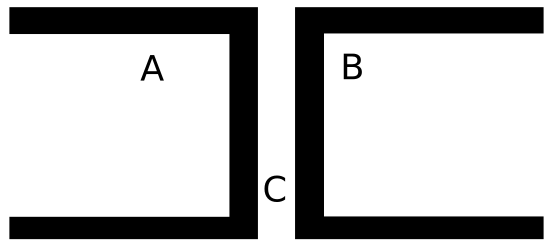
\includegraphics[width = 0.4 \textwidth]{josephson.png}
    \caption{Sketch of a Josephson junction, A and B are superconductors, while C is a barrier. The wavefunctions with respective phases $\varphi_A$ and $\varphi_B$ interfere over  C.}
    \label{figure_josephson_junction}
\end{figure}

The supercurrent flowing through the junction depends on the density of electron-electron pairs or Cooper pairs $n_{S,A}$ and $n_{S,B}$, the phases of the two macroscopic wave functions $\Psi_A$ and $\Psi_B$ and the properties of the junction. Assuming that the coupling is small, we have that $\abs{\Psi_A}^2 = n_{S,A}$ and $\abs{\Psi_B}^2 = n_{S,A}$ remain approximately constant and should have the same value $n_{S}$. 
According to \cite{grossmarx}, and from equation \eqref{supercurrent2} supercurrent density is
\begin{equation}
    \mathbf{J_s} = q n_S(\mathbf{r},t) \left[ \frac{\hbar}{m} \nabla \theta(\mathbf{r},t) - \frac{q}{m} \mathbf{A}(\mathbf{r},t) \right] = \frac{q n_S \hbar}{m} \mathbf{\gamma}(\mathbf{r},t)
\end{equation}
with $\mathbf{\gamma}(\mathbf{r},t) = \nabla \theta - \frac{2 \pi}{\Phi_0} \mathbf{A}(\mathbf{r},t)$. It is fair to assume that the phase gradient in the barrier is big compared to the gradient in the superconductor. Assuming further that the phase gradient $\mathbf{\gamma}$ is constant over the small junction, one can introduce a gauge invariant phase difference $\varphi(\mathbf{r}, t)$ as \\
\begin{equation}
    \begin{split}
        \label{eq_phase}
        \varphi(\mathbf{r}, t) &= \int^B_A \mathbf{\gamma}(\mathbf{r},t) = \int^B_A \big[ \nabla \theta - \frac{2 \pi}{\Phi_0} \mathbf{A}(\mathbf{r},t) \big] \dif \mathbf{l} \\
        &= \theta_B(\mathbf{r}, t) - \theta_A(\mathbf{r}, t) - \frac{2 \pi}{\Phi_0} \int^B_A \mathbf{A}(\mathbf{r},t) \dif \mathbf{l}.
    \end{split}
\end{equation}
According to \cite{skriptum}, the supercurrent $I_S$ solely depends on the phase difference $\varphi$. Furthermore, the wave functions $\Psi_A$ and $\Psi_B$ have to be invariant under a phase change of a multiple of $2 \pi$. 
\begin{equation}
    I_S(\varphi) = I_S(\varphi + n 2 \pi)
\end{equation}
Also, if there is no supercurrent in the superconductor, the phase difference has to be $0$. Hence, one can write 
\begin{equation}
    I_S(\varphi = 0) = 0 = I_S( n 2 \pi).
\end{equation}
Combining these results leads to a sinusodial dependence of the supercurrent $I_S$ on the phase difference $\varphi$.
\begin{equation}
    I_S(\varphi) = I_C \sin(\varphi) + \sum^{\infty}_{m = 2} I_m \sin(m \varphi) \approx I_C \sin(\varphi),
    \label{first_josephson}
\end{equation}
where $I_C$ is the critical current. Eq. \ref{first_josephson} is often referred to as the first Josephson equation. The higher order terms are often ignored as they are usually very small. \\
The second Josephson equation can be calculated from the time derivative of Eq. \ref{eq_phase}, which is 
\begin{equation}
    \pdv{\varphi}{t} = \pdv{\theta_B}{t} - \pdv{\theta_A}{t} - \frac{2 \pi}{\Phi_0} \pdv{}{t} \int^B_A \mathbf{A}(\mathbf{r},t) \dif \mathbf{l}.
\end{equation}
Using the energy-phase relation form \cite{grossmarx}, which is given as 
\begin{equation}
    -\hbar \pdv{\theta}{t} = \frac{1}{2 n_S} \Lambda \mathbf{J_s}^2 + q \phi + \mu,
\end{equation}
where $\Lambda = \frac{m}{n_S q^2}$ is the London coefficient, $q = -2 e$ is the charge of a Cooper pair, $\phi$ is a gauge scalar field and $\mu$ is the chemical potential. This yields the following expression:
\begin{equation}
    \pdv{\varphi}{t} = - \frac{1}{\hbar} \left( \frac{\Lambda}{2 n_S} \underbrace{[\mathbf{J}_s^2(B) - \mathbf{J}_s^2(A)]}_{ = 0} + q[\phi(B) - \phi(A)] + [\mu(B) - \mu(A)] \right) -  \frac{2 \pi}{\Phi_0} \pdv{}{t} \int^B_A \mathbf{A}(\mathbf{r},t) \dif \mathbf{l}
\end{equation}
Continuity requires that the currents at both sides of the junction are equal in size. This then leads to the second Josephson equation:
\begin{equation}
\pdv{\varphi}{t} = \frac{2 \pi}{\Phi_0} \int^B_A \left[ - \nabla \phi - \pdv{\mathbf{A}}{t} \right] \dif \mathbf{l} = \frac{2 \pi}{\Phi_0} \int^B_A \mathbf{E}(\mathbf{r},t) \dif \mathbf{l} = \frac{2 \pi}{\Phi_0} U,
\end{equation}
where $U$ is the voltage over the junction. It follows that the phase increases with time, resulting in 
\begin{equation}
    \varphi(t) = \varphi_0 + \frac{2 \pi}{\Phi_0} U t.
    \label{eq_josephson_2}
\end{equation}

\subsubsection*{AC Josephson Effect} % AC & Shapiro Steps
If one now adds an alternating current to the DC voltage $U = U_0 + U_1 \sin(\omega_1 t)$ in Eq. \ref{eq_josephson_2}, one gets 
\begin{equation}
    \varphi(t) = \varphi(0) + \frac{2 e U_0}{\hbar} t + \frac{2 e U_1}{\hbar \omega_1} \sin(\omega_1 t).
\end{equation}
This expression can now be inserted into the first Josephson equation, which yields 
\begin{equation}
    I_S(\varphi) = I_C \sin \left( \varphi(0) + \frac{2 e U_0}{\hbar} t + \frac{2 e U_1}{\hbar \omega_1} \sin(\omega_1 t) \right). 
\end{equation}
Using the Bessel functions $\pazocal{J}_n$, one can write this equation as
\begin{equation}
    I_S(t) = I_C \sum^{\infty}_{n = 0} \pazocal{J}_n \left[ \frac{2 e U_1}{\hbar \omega_1} \right]\sin \left( \varphi(0) + \left(\frac{2 e U_0}{\hbar} \pm n \omega_1 \right)t \right).
\end{equation}
Notice that when  $U_0 = n \frac{\hbar \omega_1}{2e}$, the sine does not depend on the time, therefore if one measures the $I$-$V$ characteristic of a Josephson junction, one will see steps in the curve. These steps are called Shapiro steps, and the width of such steps are determined by the Bessel functions.

\subsubsection*{Superconducting QUantum Interference Device - SQUID}
A simple circuit diagram of a SQUID is displayed in Fig. \ref{fig_squid}. It shows that the Josephson junctions are set up in a parallel way and are connected with superconducting material. Assuming that the critical current $I_C$ is equal for both junctions, one can use the phase-current relation from \cite{grossmarx}, which says that the currents in then junctions can be expressed as $I_{S,1}=I_C \sin(\varphi_1)$ and $I_{S,2} = I_C \sin(\varphi_2)$.
\begin{figure}[htp!]
    \centering
    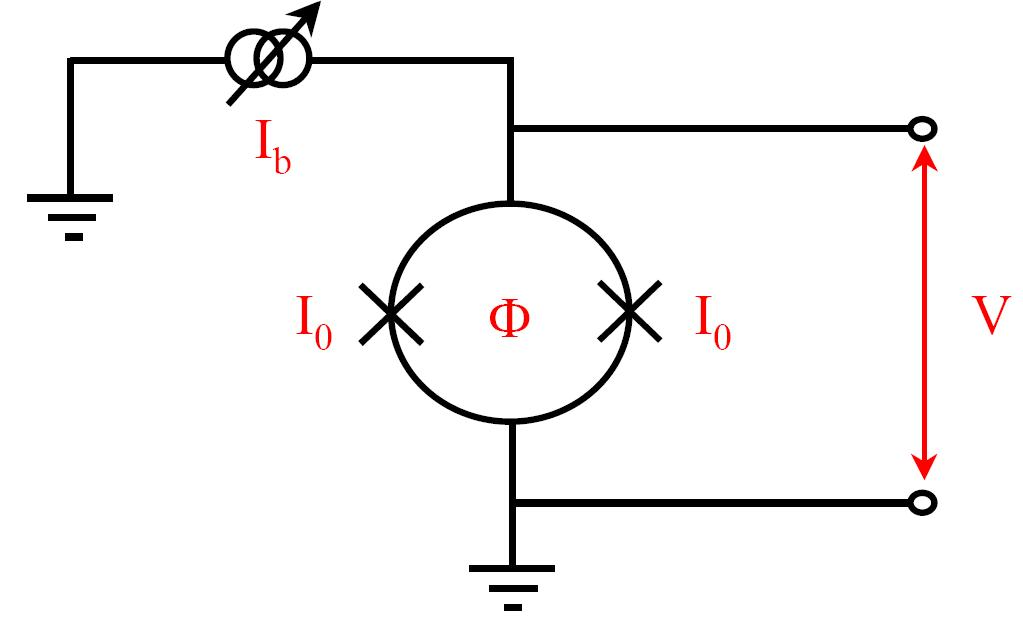
\includegraphics[width = 0.6 \textwidth]{SQUID_IV.jpg}
    \caption{Schematic of a DC SQUID, taken from \cite{squid_circuit}. An input bias current $I_b$ produces a voltage over the two parallel arranged Josephson junctions, through which a current $I_0$ is passing. If one now adds a magnetic flux $\Phi$ through the SQUID, an additional current $I_S$ is induced, which is running circular in the SQUID, adding to the bias current in the Josephson junctions. This induced current reduces the critical current of the SQUID.}
    \label{fig_squid}
\end{figure}
Using Kirchhoff's law and the addition theorems, one can write the total current as 
\begin{equation}
    \label{eq_continuity}
    I_S = I_{S,1} + I_{S,2} = 2 I_C \cos(\frac{\varphi_2 - \varphi_1}{2}) \sin(\frac{\varphi_1 + \varphi_2}{2})
\end{equation}
According to \cite{grossmarx}, one can further argue that in the total phase change across the ring, the phase change in the superconductor is negligible compared to the change in the Josephson junctions. Therefore, one can reach the following equation using Eq. \ref{eq_phase}. 
\begin{equation}
    \varphi_1 - \varphi_2 = - \frac{2 \pi}{\Phi_0} \underbrace{ \oint \mathbf{A} \dif \mathbf{l} }_{= \Phi}
\end{equation}
Here $\Phi$ is the flux through the SQUID. Inserting this into Eq. \ref{eq_continuity} leads to 
\begin{equation}
    I_S^\mathrm{max} = 2 I_C \cos(\frac{\pi \Phi}{\Phi_0}) \sin(\varphi_1 + \frac{\pi \Phi}{\Phi_0}) \stackrel{\Phi = \Phi_\mathrm{ext}}{=} 2 I_C \abs{\cos \left( \frac{\pi \Phi_\mathrm{ext}}{\Phi_0} \right)}.
\end{equation}
This equation finally shows the critical maximum that the supercurrent can reach when a magnetic field is applied on the SQUID. $I_C$ in this equation means the critical current per junction, which is half the critical current of the SQUID. 

\section{Experimental Setup}

\subsection{The $V$-$I$ characteristics}
\label{setup_vi}
The first part of the experiment was the measurement of the $V$-$I$ characteristics. In order to conduct this measurement the SQUID probe was first connected to the control box and then inserted into a bath of liquid nitrogen to cool down the probe below the critical temperature $T_c$. Measurements above $T_c$ were conducted only in the last part of the experiment. 
The lever on the control box is switched to $V$-$I$ mode, the FLUX and BIAS OFFSET are both turned into 12-o'clock position, the SWEEP OUTPUT is put at the zero position. Then the BIAS is tuned to what was estimated to be the center position in the $V$-$I$ characteristic curve on the oscilloscope. Then the SWEEP OUTPUT was gradually increased. In $V$-$I$ mode the SWEEP varies the BIAS OFFSET so one can actually see a characteristic curve on the oscilloscope. However, one has to consider that the output of the control box, which is visible on the oscilloscope is amplified by a factor of $\num{e4}$\cite{skriptum}. 
To vary the critical current one can in a final step change the FLUX OFFSET. This causes the $I_C$ to oscillate between a minimum and a maximum. For several FLUX settings the $V$-$I$ characteristics were recorded and are further discussed in the analysis.

\subsection{The $V$-$\Phi$ characteristics}
In the following part the $V$-$\Phi$ characteristics had to be recorded. Continuing from the previous setup, the FLUX setting was adjusted to where the critical current reaches a maximum. In a next step the SWEEP was put to zero, so that only a point was visible on the oscilloscope. By using BIAS, this point was positioned right at the ``knee'' of the $V$-$I$ characteristic curve. 
Next, the mode of the control box was changed to $V$-$\Phi$ mode. In this setting the SWEEP OUTPUT does not affect the BIAS but the FLUX OFFSET. One can now increase the SWEEP, which results in a sinusodial curve on the oscilloscope. These curves are saved and again displayed and discussed in the analysis.  

\subsection{Shapiro steps and $e/h$}
In order to observe Shapiro steps, we inserted an antenna into the dewar to couple the electromagnetic radiation into the SQUID. The antenna was connected to a function generator which we used to generate a sine wave with variable amplitude and frequency. With this setup we acquired again the characteristic V-I curve of the SQUID for five different frequencies ranging from 10 to 20 GHz. After setting the desired frequency we changed the power of the wave such that the Shapiro steps were maximized.
\subsection{Critical temperature measurement}
To measure the critical current of the SQUID we measured the resistance at various temperatures. To determine the temperature we built the circuit in figure \ref{circuit}. The REF02 provides us with a stable voltage of approximately 5V, we chose resistor $R_1 \simeq 40$ k$\Omega$ and $R_2 \simeq 10$ k$\Omega$ such that the voltage at the non inverting input of the opamp is around 1V. For the last resistor  we chose $R_3 \simeq 80$ k$\Omega$, thus the fixed current was approximately 12 mA. The diode was attached to the SQUID, hence we were able to measure a difference in temperature by measuring the voltage across the diode. To calibrate this circuit we took two points, one at the boiling point of the nitrogen (77 K) and the other one at room temperature, such that we had a direct conversion from voltage to temperature.\\
To measure the resistance of the SQUID we acquired the characteristic V-I curve whose slope gives its resistance. We proceeded to slowly lower the SQUID into the liquid nitrogen, such that the gradient of temperature between the liquid nitrogen and the environment would give us different points with different temperatures. During the lowering we stopped several times to take the measurements, every time we waited for several minutes until voltage on the multimeter was stable and then we acquired the resistance and wrote down the voltage of the multimeter.
We took several points with different spacing, more densely near the critical temperature at 90 K and more rarely at higher temperature until the SQUID was completely submerged in the liquid nitrogen and therefore at 77 K.
\begin{figure}[H]
\centering
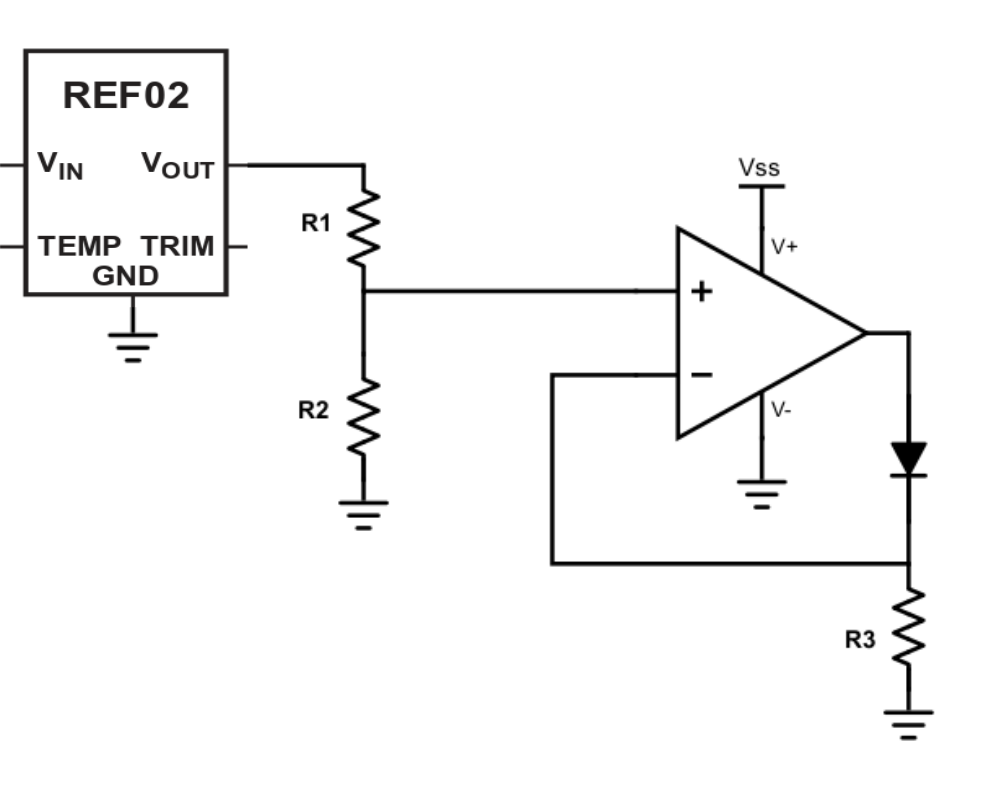
\includegraphics[width = .5\textwidth]{circuit}
\caption{Circuit for current source used to measure the temperature}\label{circuit}
\end{figure}

\section{Analysis}
Before starting to analyse the data, one has to decide how to extract useful data points. The problem is that the oscilloscope saves VOLTAGE and CURRENT OUTPUT in two independent files, in which also the time of the measurement point is noted. Due to the SWEEP OUTPUT we get multiple lines from left to right and vice versa, so we exploited this excess of data to smooth the lines and calculate an error for every point. First we sorted the data in ascending order according to their respective $x$ axis value (usually the current). Then we averaged over 10 neighboring points. The final curve is the set of all the averages and the standard deviation used as an error. This has been done for all the data analysed in the next three sections.
\subsection{The $V$-$I$ characteristics}
As was already described in Sec. \ref{setup_vi}, the characteristic $V$-$I$ curve was measured in the first part of the experiment. Fig. \ref{fig_iv_characteristics} displays two $V$-$I$ characteristics. The left curve shows the maximum value of $I_C$ that was measured during the experiment, which means that the flux was at that point close to an integer multiple of the fluxon $\Phi_0$. To the right one can see the minimized $I_C$, which corresponds to an integer plus $1/2$ multiple of $\Phi_0$. \\
\begin{figure}[htp!]
    \centering
    \begin{subfigure}[t]{0.45 \textwidth}
        \centering
        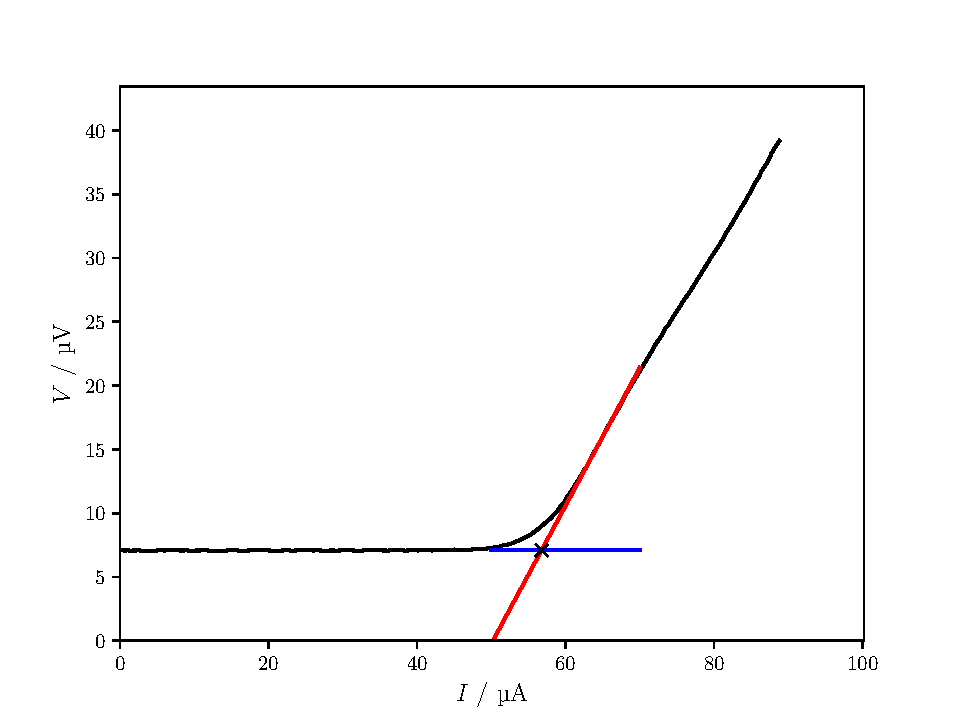
\includegraphics[height=6cm]{iv_max.pdf}
        \caption{ }
    \end{subfigure}
    ~ 
    \begin{subfigure}[t]{0.45 \textwidth}
        \centering
        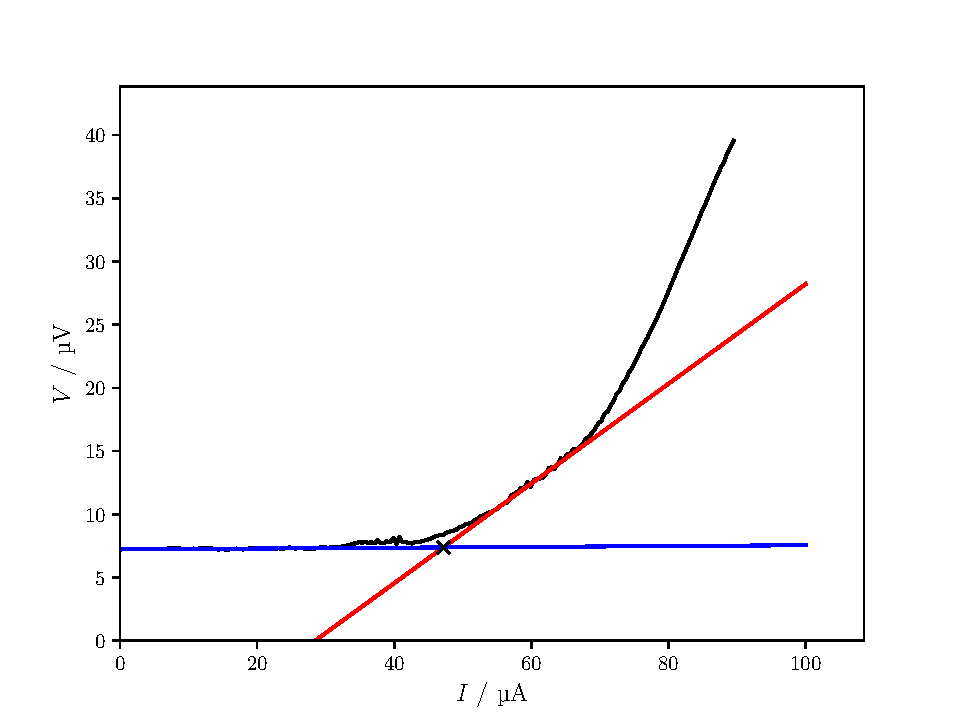
\includegraphics[height=6cm]{iv_min.pdf}
        \caption{ }
    \end{subfigure}
    \caption{Measured $V$-$I$ characteristics for an integer and an integer plus $1/2$ magnetic flux. The parameters of the linear functions are listed in Tab. \ref{tab_iv_characteristics}. The resulting critical currents are $I_C^{max} = \SI{56.8(8)}{\micro \ampere}$ and $I_C^{min} = \SI{47.2(17)}{\micro \ampere}$. }
    \label{fig_iv_characteristics}
\end{figure}
\begin{table}[htp!]
    \caption{List of the fit parameters from Fig. \ref{fig_iv_characteristics}. The fitted function was $V = a I + b$. }
    \centering
    \begin{tabular}{l | l | l | l}
        max/min $I_C$ & color & $a$ & $b$ \\ \hline
        $I_C^{max}$ & red & \SI{1.082(11)}{\ohm} & \SI{-54.3(7)}{\micro \volt} \\ 
        $I_C^{max}$ & blue & \SI{0.0006(109)}{\ohm} & \SI{7.1(7)}{\micro \volt} \\
        $I_C^{min}$ & red & \SI{0.394(9)}{\ohm} & \SI{-11.2(5)}{\micro \volt} \\
        $I_C^{min}$ & blue & \SI{0.00328(19)}{\ohm} & \SI{7.230(3)}{\micro \volt}
    \end{tabular}
    \label{tab_iv_characteristics}
\end{table}
From the fit parameters the critical currents are deduced as $I_C^{max} = \SI{56.8(8)}{\micro \ampere}$ and $I_C^{min} = \SI{47.2(17)}{\micro \ampere}$. From the difference between these two values, one can derive the screening current as $I_S = I_C^{max} - I_C^{min} = \SI{9.6(19)}{\micro \ampere}$. \\
To determine the normal resistance $R_n$ one takes a data set with a wide range of $I$ values as depicted in Fig. \ref{fig_resistance}. The slope of the linear fit across the data corresponds to the normal resistance $R_n = \SI{0.6747(2)}{\ohm}$, which is reasonably close to the \SI{0.64}{\ohm} that are given in the data sheet.\cite{datasheet} \\
\begin{figure}[htp!]
    \centering
    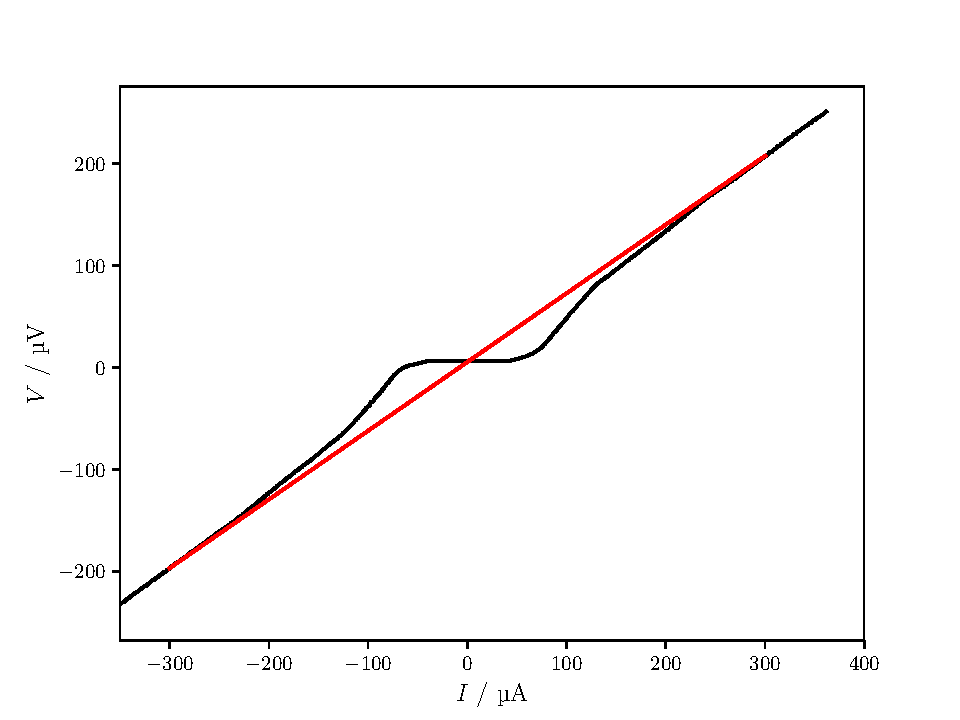
\includegraphics[width = 0.6 \textwidth]{resistance.pdf}
    \caption{Wide range $V$-$I$ characteristic curve. From the linear fit with parameters $a = \SI{0.6747(2)}{\ohm}$ and $b = \SI{5.36(7)}{\micro \volt}$ the resistance $R_n = a$ can be deduced.}
    \label{fig_resistance}
\end{figure}
To finalize the analysis of the first part, we had to calculate the modulation parameter $\beta_L$ in three different ways, that are all precisely outlined in \cite{skriptum}. In short, the modulation parameter reveals to which extent the SQUID is able to hold the flux constant by generating a circular current. Furthermore, it holds information on the SQUID's flux-to-voltage transfer ratio. 
\\
All necessary equations are listed below. As one will notice, the second and the third equations are very similar to each other. Essentially, the difference is that the third one also accounts for effects like thermal noise. Thermal effects may not be so important for low-temperature superconductors, but since the Mr. SQUID probe is held at comparably high \SI{77}{\kelvin} (boiling temperature of molecular nitrogen) one will see that thermal effects are important to consider. 
\begin{equation}
    \label{beta_1}
    \beta_{L,1} = \frac{2 L I_C}{\Phi_0}
\end{equation}
\begin{equation}
    \label{beta_2}
    \beta_{L,2} = \frac{4 I_C R_n}{\pi \Delta V} - 1
\end{equation}
\begin{equation}
    \label{beta_3}
    \beta_{L,3} = \frac{4 I_C R_n}{\pi \Delta V} \left( 1 - 3.57  \frac{\sqrt{k_B T L}}{\Phi_0} \right) - 1
\end{equation}
Here, $L$ is the inductance of the Mr. SQUID probe, which is estimated to be \SI{73}{\pico \henry} in \cite{skriptum}. $I_C$ and $R_n$ are known from the $V$-$I$ characteristics and the measurement of the resistance. Finally, $\Phi_0$ represents a fluxon. Since $\Delta V$ describes the maximum modulation depth of the $V$-$\Phi$ characteristic curve, the result for Eq. \ref{beta_2} and \ref{beta_3} will be given in Sec. \ref{sec_v_phi}. 
\\
Using the mentioned values for $L$, $\Phi_0$ and Eq. \ref{beta_1} one arrives at $\beta_{L,1} = \num{4.01(6)}$. 

\subsection{The $V$-$\Phi$ characteristics}
\label{sec_v_phi}
In the second part of the experiment several $V$-$\Phi$ curves were recorded, a more thorough description of the conduction of the experiment is given in the description of the experimental setup. Fig. \ref{fig_iphi_characteristics} shows the dataset with the highest amplitude of the oscillation. The most interesting results are the modulation depth $\Delta V = 2 a = \SI{5.748(6)}{\micro \volt}$ and the period of the function $\Delta I = 2 \pi / b = \SI{96.44(3)}{\micro \ampere}$. 
\begin{figure}[htp!]
    \centering
    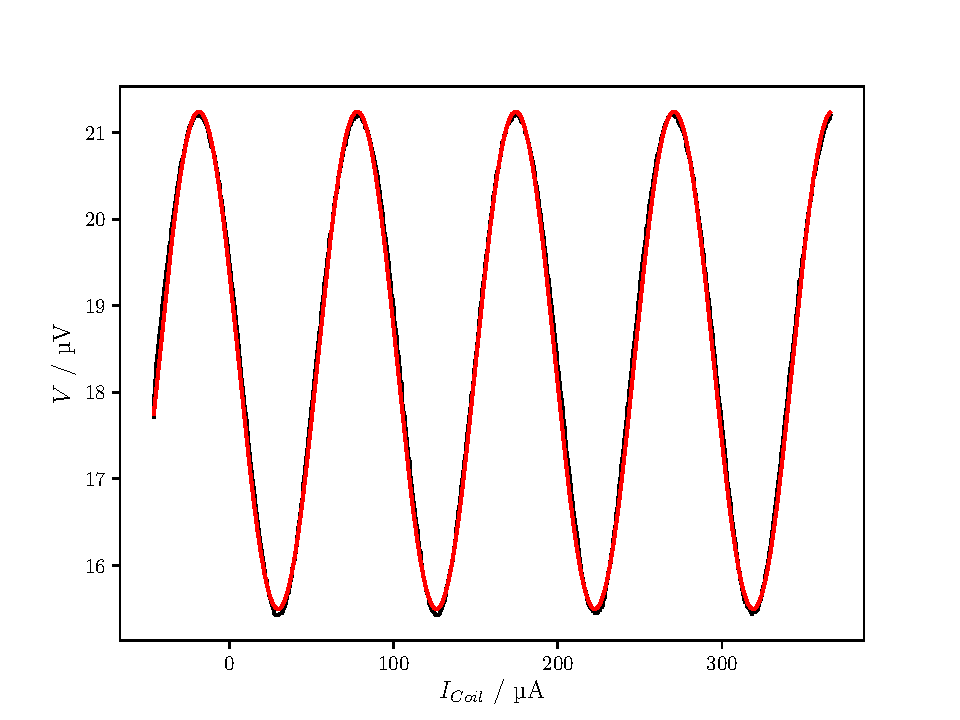
\includegraphics[width = 0.6 \textwidth]{v_flux.pdf}
    \caption{Plot with measured data (black) and fitted function (red). The function used was $V = a \sin(b I_{Coil} + C) + d$, which yielded parameters of $a = \SI{2.874(3)}{\micro \volt}$, $b = \SI{0.06515(2)}{\per \micro \ampere}$, $c = \num{2.777(3)}$ and $d = \SI{18.369(3)}{\micro \volt}$.}
    \label{fig_iphi_characteristics}
\end{figure}
\\
Starting with $\Delta V$, one can now calculate $\beta_L$ with Eq. \ref{beta_2} and \ref{beta_3}, which leads to 
\begin{equation*}
    \begin{split}
        \beta_{L,2} &= \num{7.49(12)} \\
        \beta_{L,3} &= \num{3.41(6)}
    \end{split}
\end{equation*}
While both values disagree with $\beta_{L,1}$, which was calculated from the definition of the modulation parameter, one also notices that the value for $\beta_{L,3}$ is by far closer to $\beta_{L,1}$ than $\beta_{L,2}$. This was to be expected, since $\beta_{L,3}$ takes thermal effects into account.
\\ % coupling of the coil
Next, one is looking for the coupling of the internal coil, which was used to generate the flux in the $V$-$\Phi$ curve. Because the induced current in the SQUID is equal for $\Phi = n \Phi_0$ and $\Phi = (n + 1) \Phi_0$, but not for $\Phi = (n + 1/2) \Phi_0$, one can say that after one period in Fig. \ref{fig_iphi_characteristics} the flux has increased by exactly one fluxon. This means that the coupling constant $C$ would be $\Delta I / \Phi_0 = \SI{96.44(3)}{\micro \ampere} / \Phi_0$. The corresponding value in the data sheet \cite{datasheet} is given as $\SI{98}{\micro \ampere} / \Phi_0$, which means that our measurement is close. The margin is likely due to limited experience in fully optimizing all the settings on the control box of the SQUID, and different setup condition: in \cite{datasheet} the experiment is carried out at 75 K for example.
\\
Furthermore, one can calculate the mutual inductance $M$ of the internal feedback coil, which is essentially the inverse of the coupling constant as Eq. \ref{eq_inductance} shows. 
\begin{equation}
    \label{eq_inductance}
    M = \frac{\Phi_0}{\Delta I} = \SI{2.144(7)e-11}{\henry}
\end{equation}
Again, this is a little less than the value listed in \cite{skriptum}, which claims that the mutual inductance of internal coil of the Mr. SQUID probe is \SI{23}{\pico \henry}. \\
% Here comes the flux sensitivity
Next, a look is taken at the flux sensitivity of the SQUID, meaning the smallest measurable change in the measured flux. Here, it is essential to know the noise in the setup. The noise in the voltage $\delta V$ is estimated by calculating the standard deviation of every data point from the fit function in Fig. \ref{fig_iphi_characteristics}. Then it is assumed that the relation to the noise in the current $\delta I$ is 
\begin{equation}
    \begin{split}
        \label{eq_noise}
        \frac{\delta V}{\delta I} &= \frac{\dif V}{\dif I} \\
        \delta I &= \frac{\delta V}{\frac{\dif V}{\dif I}}. 
    \end{split}
\end{equation}
The plot of $\delta I$ can be seen in Fig. \ref{fig_noise}. As one can see, the minima in the noise of the current, which is proportional to the flux, are placed where the slope of the $V$-$\Phi$ curve is very steep. That the setup is most sensitive at the steepest slopes appears to be reasonable, since a small change in the flux would cause a bigger change in voltage the steeper the slope is. The minimum value that is reached is $\delta I_\mathrm{min} = \SI{1.56(2)}{\micro \ampere}$, which would correspond to a flux of $\Phi = (\num{0.0162(2)}) \Phi_0$. Fig. \ref{fig_noise} also shows singularities, which appear whenever the cosine in Eq. \ref{eq_noise} is equal to zero. Of course these singularities are not physical, but appear because of the derivative used in Eq. \ref{eq_noise}. Since the maximum or minimum turning points in the $V$-$\Phi$ curve are not so interesting for the maximum of sensitivity, the sensitivity at the high/low turning points was graphically estimated to be roughly \SI{7}{\micro \ampere}. 
\\
According to \cite{drung} and \cite{kleiner}, contemporary DC SQUIDs can measure changes in flux up to about $\num{e-6} \Phi_0$. This is approximately four magnitudes better than the measurement conducted in this experiment. 
\begin{figure}[htp!]
    \centering
    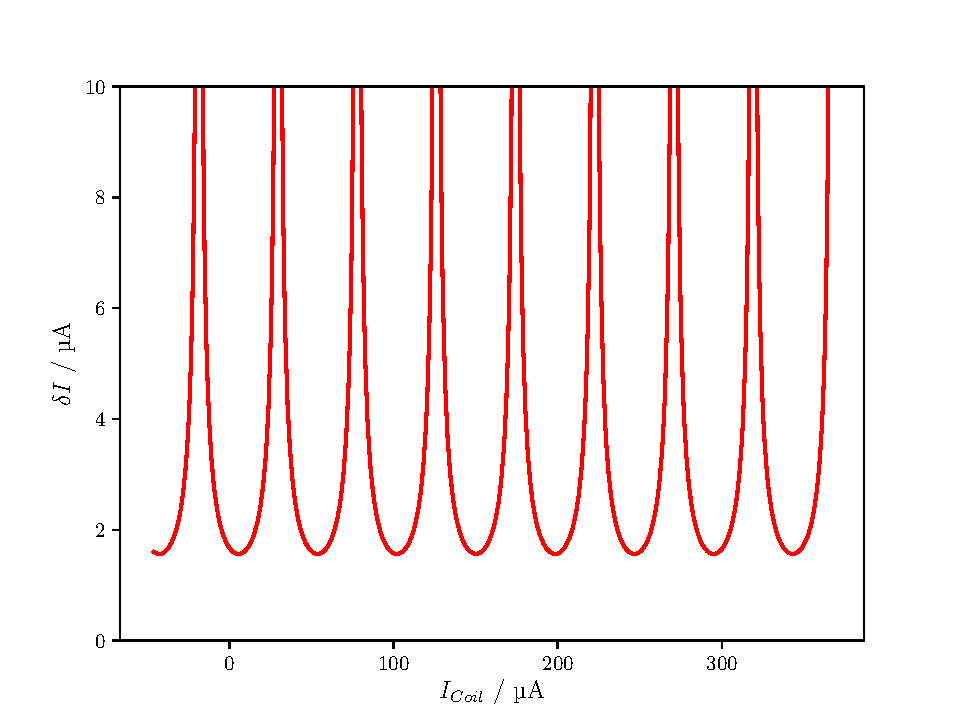
\includegraphics[width = 0.6 \textwidth]{noise.pdf}
    \caption{Depiction of the change in the current $\delta I$ that we can measure.}
    \label{fig_noise}
\end{figure}

\subsection{Shapiro steps and $e/h$}
\begin{figure}[H]
\centering
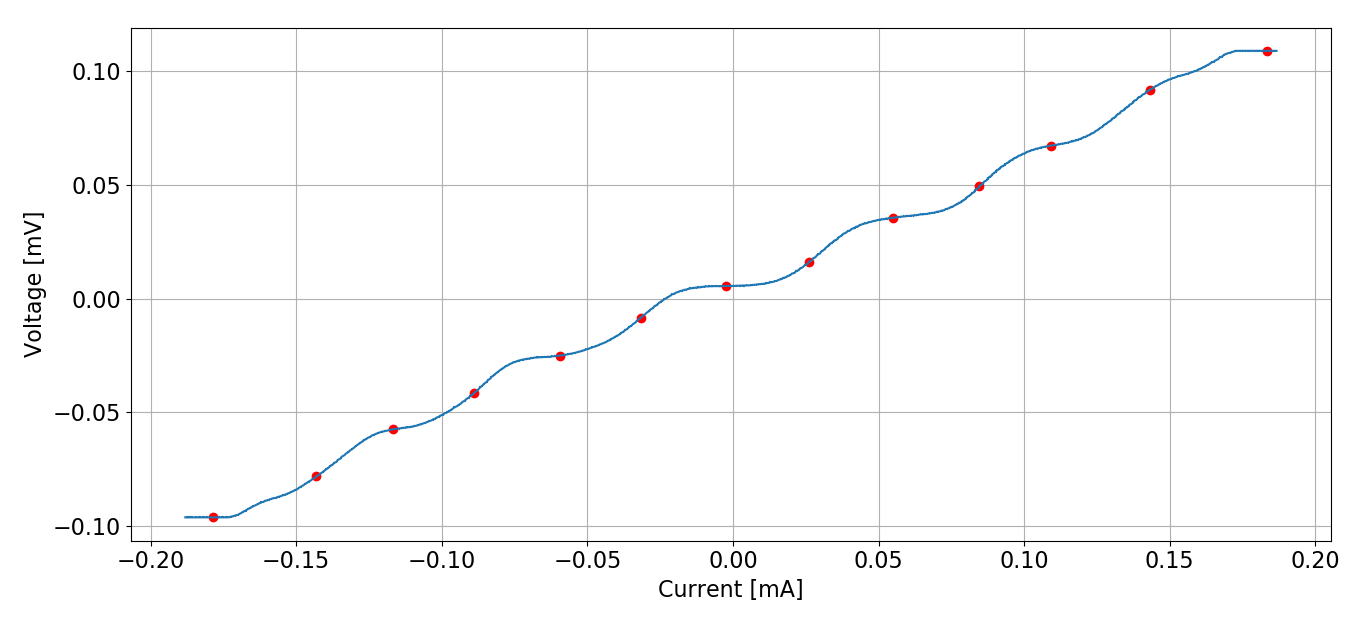
\includegraphics[width = \textwidth]{shapirosteps}
\caption{Shapiro steps for frequency of 15 GHz, red points are the calculated inflection points. Errors are too small to be seen.}\label{shapiro}
\end{figure}
An example of acquired data is shown in figure \ref{shapiro}. The goal of the analysis is to find the steps in the curve, a non-trivial task. We identify a step as an inflection point in our data. The approach we used to find the inflection point was to interpolate the data with a spline for which it is easy to find the inflection point. Then after finding the inflection points on the spline, we took the closest points of the data to the calculate inflection points. The result of this algorithm can be seen in figure \ref{shapiro}.\\
To calculate the step height we took as many steps as possible for every frequency, calculated the difference in height between these steps and then divided by the number of steps taken, such that the error is minimized. The step height for every frequency can be seen in figure \ref{eh}, the error is calculated with propagation on the difference between two point and then is divided by the number of steps taken. From the theory we know that the height of one step should be
\begin{equation}U_0 = \frac{h\nu}{2e},\end{equation}
hence, we did a linear regression on the data in figure \ref{eh} to find the slope $h/2e$. The point at 20 GHz was excluded since it is several standard deviations aways from what we expected, likely due to an unknown error or maybe a problem in the inflection point detection algorithm. The regression gave the value $0.00208\pm 0.8\cdot 10^5$ mV for the slope with a reduced chi squared of $\chi_\nu \simeq 75$, thus we find $e/h = 24010 \pm 930$ GHz/V, where the error is calculated through propagation. The literature value for $e/h$ is $ 2.4179671\cdot 10^{14}$ Hz/V \cite{skriptum}, which is compatible with what we found. The regression has a very high $\chi_\nu$, but this could be caused by low statistics, in fact the regression has only two degrees of freedom.
\begin{figure}[H]
\centering
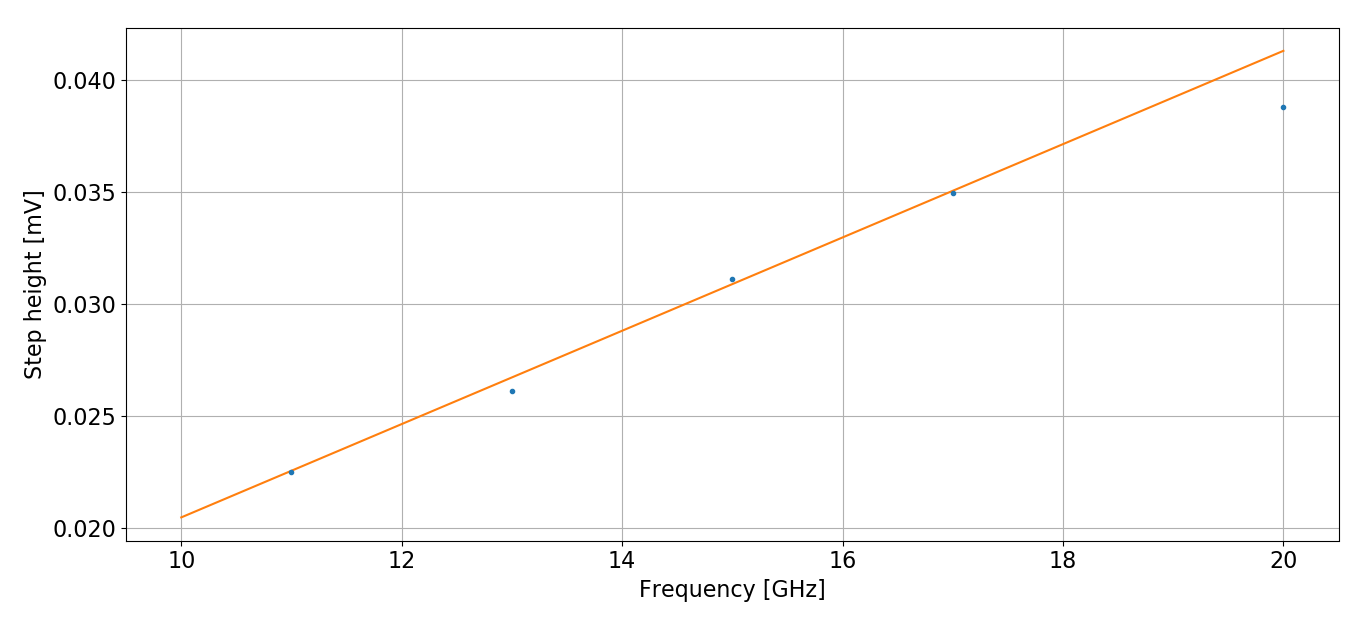
\includegraphics[width = \textwidth]{eh}
\caption{Step height as a function of frequency, orange line is the linear regression. Errors on the points are too small to be seen.}\label{eh}
\end{figure}
\subsection{Critical temperature measurement}
\begin{figure}[H]
\centering
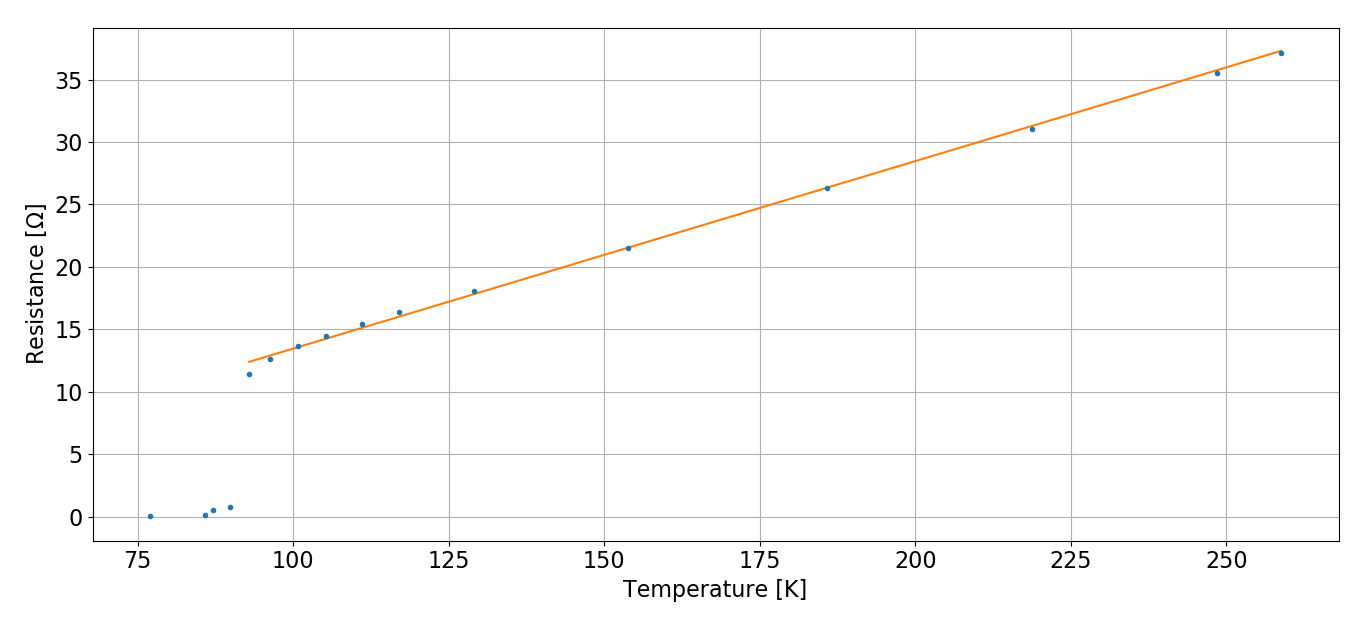
\includegraphics[width = \textwidth]{img/tempR.png}
\caption{Resistance of the SQUID as a function of temperature, data above 90 K has been fitted with a line: slope: $0.150\pm 0.003$ 1/K, intercept: $-1.5\pm0.4\,\Omega$.}\label{resistance}
\end{figure}
The calibration of the circuit was done with two points at 77 K and room temperature, with these two values we calculated the parameters of a line $y=ax+b$, such that we could convert from diode voltage to temperature. We cut the acquired characteristic curve around zero current, then we fitted the data with a line and the slope gave us the resistance of the SQUID. An example of acquired data with fit is shown in Fig. \ref{92}. Finally the curve in Fig. \ref{resistance} was produced for the measured temperatures. We can clearly see a drop in the resistance around 90 K. 
At 92 K the measured resistance is $11.45 \pm  0.01 \, \Omega$ , while at 89 K $0.76\pm 0.03\, \Omega$ which is two orders of magnitude lower, but still not 0. At 77 K, the resistance is
$0.01\pm 0.07\, \Omega$, which is essentially 0. We guess that the real critical temperature is between the point at 89 K and 92 K, even if at 89 K the resistance is not perfectly 0, but as can be seen in figure \ref{89} under 90 K we have a problem of hysteresis in our data. Moreover, small systematic errors could easily raise this resistance and bring it off from 0. Therefore, we conclude from our data that the critical temperature is $T_c = 90.5 \pm 1.5$ K, which is the interval between the two aforementioned temperatures. This value is in agreement with the measured critical temperature of a pure $\text{YBa}_2\text{Cu}_3\text{0}_7$ crystal ($\approx 90.5$ K) \cite{criticaltemperature}.
\begin{figure}[H]
\centering
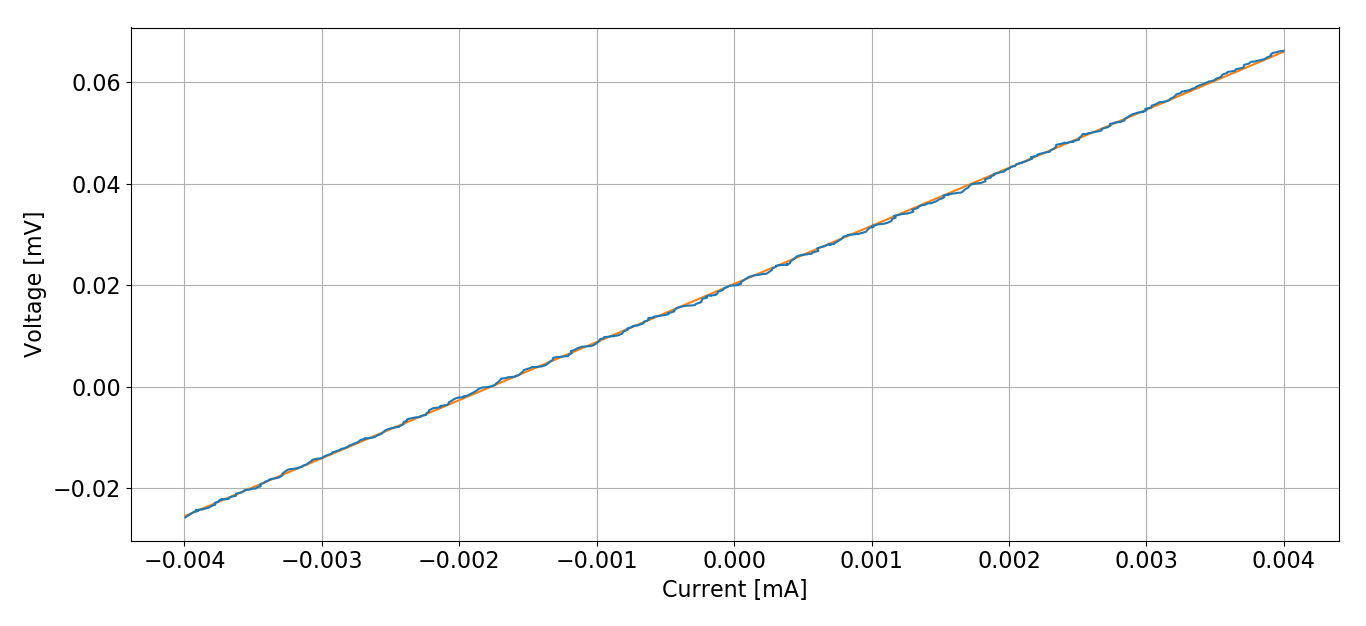
\includegraphics[width = \textwidth]{92K}
\caption{Characteristic curve of the SQUID at 92 K.}\label{92}
\end{figure}
\begin{figure}[H]
\centering
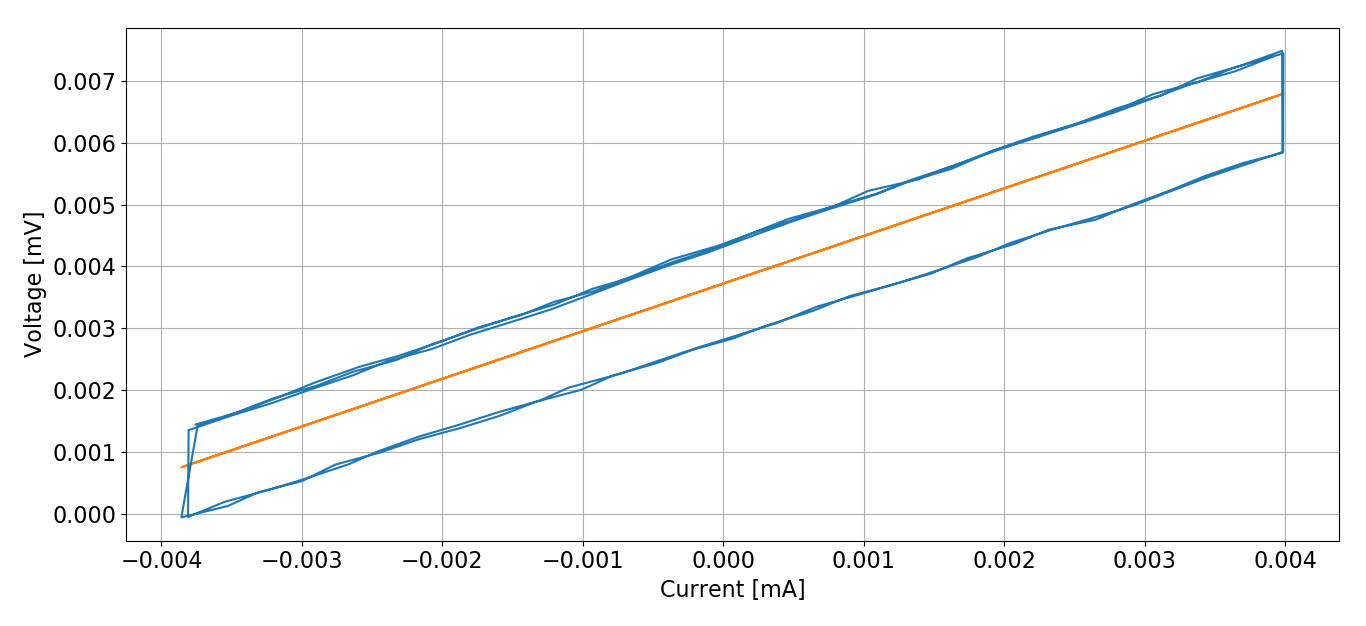
\includegraphics[width = \textwidth]{89K}
\caption{Characteristic curve of the SQUID at 89 K.}\label{89}
\end{figure}
\section{Conclusion}
In this experiment we explored the features of a SQUID device, along with studying several properties of superconductors. The most remarkable results obtained are the small sensitivity in detecting flux change: $10^{-2} \Phi_0$ that is $10^{-17}$ Wb, and we found the critical temperature of the superconductor YBCO $\approx 90.5$ K. However, this last result could be affected 
by systematic errors, for instance: the temperature was measured with a diode, which was close to the SQUID, but probably the temperature of the diode and the SQUID could have been slightly different, especially near the liquid nitrogen where the temperature gradient is greater. Furthermore, the SQUID could have not been completely thermalized when we took the measure, the voltage on the multimeter was always fluctuating slightly. Another source of systematic error could be the hysteresis we had at low temperature, as already pointed out in the analysis.


\begin{thebibliography}{99}
\bibitem{firstsuperconductor} \textsc{H. K. Onnes} \textit{The resistance of pure mercury at helium temperatures}, Commun. Phys. Lab. Univ. Leiden, Vol. 12 (1911), 120 

\bibitem{skriptum}
STAR Cryoelectronics, \textit{Mr. SQUID User's  Guide}. \textsc{Randy W. Simon, Michael J. Burns, Mark S. Colclough, Greg Zaharchuk, Robin Cantor}. 

\bibitem{grossmarx}
De Gruyter Studium, \textit{Festkörperphysik}. \textsc{Rudolf Gross, Achim Marx}. 3. Edition.

\bibitem{squid_circuit}
Wikimedia, \textsc{Jan Olaf}. \url{https://upload.wikimedia.org/wikipedia/commons/7/71/SQUID_IV.jpg}.

\bibitem{datasheet}
STAR Cryoelectronics, \textit{Mr. SQUID Datasheet}. \textsc{R. Cantor}. 

\bibitem{criticaltemperature}
  \textsc{S.S. Tinchev}, \textit{Interface superconductivity {\textendash} Possible origin of high critical temperature in layered superconductors}, Physica C: Superconductivity vol 470 15-16, pag 626-629, Aug 2010

\bibitem{fluxquantization}
\textsc{S. Gasiorowicz}, \textit{Quantum physics}, 3rd ed., Wiley-VCH, (2003).

\bibitem{magneticfluxquantum}
\textit{The NIST Reference on Constants, Units, and Uncertainty} US National Institute of Standards and Technology. June 2015. 

\bibitem{drung}
IEEE TRANSACTIONS ON APPLIED SUPERCONDUCTIVITY, VOL. 17, NO. 2, JUNE 2007, \textsc{D. Drung, C. Aßmann, J. Beyer, A. Kirste, M. Peters, F. Ruede, Th. Schurig}. \textit{Highly Sensitive and Easy-to-Use SQUID Sensors}

\bibitem{kleiner}
\textsc{Reinhold Kleiner, Dieter Koelle, Frank Ludwig, John Clarke}. \textit{Superconducting Quantum Interference Devices: State of the Art and Applications} \url{https://pdfs.semanticscholar.org/460d/6375438fa069b8ada6bfcbcd8b0af37f70e2.pdf}

\end{thebibliography}
\end{document}
